\lab{Application}{Image Processing and Filters}{Image Filters}

\objective{Explore Image Filters. In particular, we will explore the Sobel Filter, which uses 
numerical derivatives to find edges in images.}
One of the primary tools in image processing is the use of filters to identify important information 
in images. In this section we will implement our own filters and explore applications.

One of the easiest filters to implement is matrix based. In this implementation, the filter that we 
select is a matrix, which represents how much we want certain pixels to contribute to the output image. 
Suppose that we choose our filter to be:

\[
A = \begin{pmatrix}
a_{-1,-1}&a_{-1,0}&a_{-1,1}\\
a_{0,-1}&a_{0,0}&a_{0,1}\\
a_{1,-1}&a_{1,0}&a_{1,1}
\end{pmatrix}.
\]

We will call our input image $B$ and our output image $C$ (both images are represented as matrices).
Our matrix filter operates according to the following formula:
\[
C_{ij} = \sum_{k=-1}^1 \sum_{m=-1}^1 a_{km}B_{i+k,j+m}.
\]

Essentially this computes each pixel of the output image as the weighted sum of the surrounding
pixels in the input image. The technical term for this type of operation is a convolution.

Suppose that our image $B$ is an $m\times n$ matrix. Note that the definition for
$C_{ij}$ given above does not make sense when $i = 0, m-1$ or $j = 0, n-1$, since we would be trying
to access matrix elements $B_{-1,j}, B_{m,j}, B_{i,-1},$ or $B_{i,n}$, which are out of bounds.
%One fix is to treat these out-of-bounds elements as copies of the nearest in-bounds element.
%That is, define
%\begin{align*}
%B_{-1,j} &:= B_{0,j},\\
%B_{m,j} &:= B_{m-1,j},\\
%B_{i,-1} &:= B_{i,0},\\
%B_{i,n} &:= B_{i,n-1}.
%\end{align*}
%For the corners, define
%\begin{align*}
%B_{-1,-1} &:=B_{0,0},\\
%B_{m,-1}&:= B_{m-1,0},\\
%B_{-1,n}&:=B_{0,n-1},\\
%B_{m,n}&:=B_{m-1,n-1}.
%\end{align*}
One fix is to assign the value of 0 to these out-of-bounds elements. This process is know as \emph{padding}
the image with zeros. The amount of padding necessary is dependent on the size of the filter.
In the following code, we create a padded version of the image $B$ with respect to a filter $f$ of shape 
$h\times k$, where we assume that $h$ and $k$ are odd integers.

\begin{lstlisting}
>>> import numpy as np
>>> # assume that the matrix B and filter f already exist.
>>> # create padded version of B.
>>> m, n = B.shape
>>> h, k = f.shape
>>> B_pad = np.zeros((m + h - 1, n + k - 1))
>>> B_pad[h/2:h/2 + m, k/2:k/2 + n] = B
\end{lstlisting}

We can now easily calculate a given element of the filtered image $C$ as follows:
\begin{lstlisting}
>>> C[i,j] = (f*B_pad[i:i + h, j:j + k]).sum()
\end{lstlisting}

Make sure that you understand why this Python code does what we want it to do.
\begin{problem}
Write a function \li{Filter} that takes an image and an arbitrary filter matrix, and outputs the
filtered image. Note that for these filters to be meaningful, the number of columns and number 
of rows need to be odd (there are ways to deal with even size filters, but we won't handle them here).
\end{problem}

So what can we do with these filters? We will show an example of how to apply a Gaussian blur 
using this type of filter. You will also be able to test your code with this example. 
To begin, load the following picture:

\begin{lstlisting}
>>> import numpy as np
>>> from matplotlib import pyplot as plt
>>> K = plt.imread('cameraman.tif')
>>> plt.imshow(K, cmap = plt.cm.Greys_r)
>>> plt.show()
\end{lstlisting}

This code should display an image like the one shown in Figure \ref{imfil:camclean} (provided
that you have the correct image file, of course).

\begin{figure}
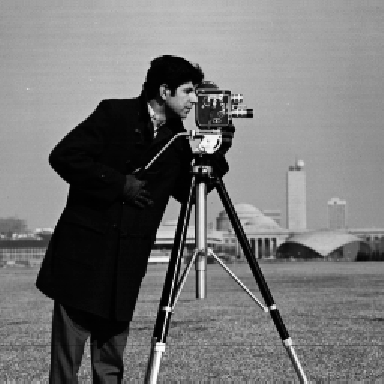
\includegraphics{cameramanClean.pdf}
\caption{An example image.}
\label{imfil:camclean}
\end{figure}

Now that you have a simple filter function, try the following filter on this image:

\[
A = \frac{1}{159}\begin{pmatrix}
2&4&5&4&2\\
4&9&12&9&4\\
5&12&15&12&5\\
4&9&12&9&4\\
2&4&5&4&2
\end{pmatrix}
\]

\begin{lstlisting}
>>> A = np.array([[2,4,5,4,2],
                 [4,9,12,9,4],
                 [5,12,15,12,5],
                 [4,9,12,9,4],
                 [2,4,5,4,2]])/159.
>>> C = Filter(K, A)
>>> plt.imshow(C, cmap = plt.cm.Greys_r)
>>> plt.show()
\end{lstlisting}
You should get an output that looks something like Figure \ref{imfil:camblur}.
\begin{figure}
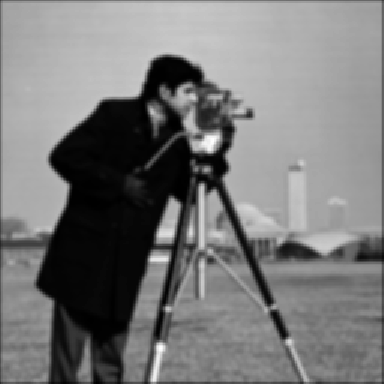
\includegraphics{cameramanBlur.pdf}
\caption{A blurred version of Figure \ref{imfil:camclean}.}
\label{imfil:camblur}
\end{figure}
You can see that the filter blurred the image. This can be very important in trying to 
wash out images that are ``noisy.''

We now turn our attention to the problem of edge detection. Automatically detecting edges in an image
can be useful in segmenting the image, detecting and extracting certain features in the image, and
sharpening contrast in the image. There are many approaches to this problem, and in this lab, we will
design a filter that numerically approximates the gradient of the image at each pixel. The magnitude
of the gradient tells us the local rate of change of the pixel values, and so large magnitudes 
correspond to regions of high contrast in the image. Since there is high contrast at edges within
the image, we have reason to hope that this approach will be effective.

The filter we will use is called the \emph{Sobel Filter}. To find the gradient 
in the vertical direction, the filter is given by:
\[
A = \frac{1}{8}\begin{pmatrix}
-1&-2&-1\\
0&0&0\\
1&2&1
\end{pmatrix}
\]
The filter for the horizontal gradient is simply the transpose of the above matrix.

For an image $B$, suppose that filtered images using the Sobel filter in the vertical and
horizontal directions are given by $B_y$ and $B_x$, respectively. These two matrices give
the $y$ and $x$ components of the gradient, respectively, at each pixel. To obtain the 
magnitude of the gradient (i.e. the length of the gradient vector), we use the formula
$$
B_{grad} = \sqrt{B_x^2 + B_y^2},
$$
where the square root and squaring operations are performed pointwise on the matrices. 
The matrix $B_{grad}$ now gives the magnitude of the gradient at each pixel, and so we
can threshold this matrix to isolate the pixels with the largest gradient, setting all 
other pixel values to 0. 
In Python, this can be done as follows:
\begin{lstlisting}
>>> B_edges = B_grad > thresh
\end{lstlisting}
where \li{thresh} is some positive threshold value of our choosing. In general, a reasonable
value for this threshold is $4\mu(B_{grad})$, where $\mu(B_{grad})$ is the mean value of the 
matrix $B_{grad}$.
If we now plot the matrix \li{B_edges}, we will see a black-and-white image with the edges 
shown as white lines.

\begin{problem}
Write a function \li{plotEdges} that finds and plots the edges of an image using the Sobel filter.
The function should take an image, and the last line of code should be a call 
to \li{plt.show}. The function should not return anything. For your threshold value, use the 
suggestion given above.

For the cameraman example, you should obtain an output similar to that displayed in 
Figure \ref{imfil:edges}.
\end{problem}

\begin{figure}[h!]
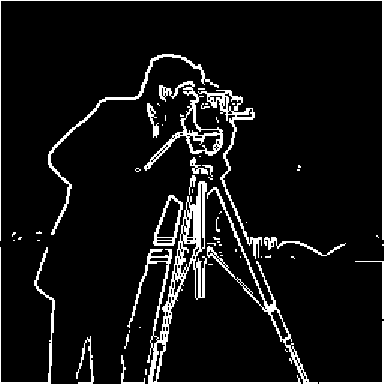
\includegraphics{edges.pdf}
\caption{A filtered version of Figure \ref{imfil:camclean}.}
\label{imfil:edges}
\end{figure}
